\section{Abstract \small\textit{Kristoffer}}
\vspace{3mm}
The idea of fully autonomous cars, has been a part of the futuristic idea of growing in peoples heads as long as such ideas has existed. Such self-driving cars use sensors to navigate the terrain and environment at which the agent finds itself in.
In this project we will be using the same principles to make the agent navigate in a given environment. 

The general problem that using these sensors face, is the amount of training time needed for the q learning algorithm to teach an agent to be self driven. The training time and the quantity of sensors correlate exponentially, and therefore too many sensors would require a long time.Whereas, an insufficient sum of sensors would leave an incomplete algorithm as it would lack the data to be fully self driven. In this project we will be comparing the sensors configuration and sum, and how these factors correlate with the agents ability to finish the track. We test 3 configurations of sensors in this article to find out which of these will perform the best.
\vspace{5mm}

\section{Introduction \small\textit{Kristoffer}}
\vspace{3mm}
Self driving cars is very much an ongoing topic regarding the future world, an has many benefits with it. Fully autonomous cars could potentially get rid of the long travel time by eliminating traffic jams, and getting rid of the long queues in the rush hours. Furthermore, they also have the ability to majorly leave a dent in the amount of car related accidents. We have already begun to see some form of autonomous cars driving on the road in Elon Musk's Tesla cars, and people can begin to imagine what problems the fully self driving car would hold of benefits. 

In the Tesla cars, they operate by using senors that shoot out from the car and use these sensors to feed the central computer, the distance between the object that the sensors hit, and the car itself. determining how far it is from objects. Other than that, the cars also use visual feedback from cameras on board to identify what object are around said car. A question to be asked here is how many sensors should a self driven car have to be able to drive perfectly, without it having to many sensors and therefore feeding the car way to much data to be able to train properly. 

In our project, we aim to come closer to how these sensors affect the ability for the car to drive smoothly around a racetrack. We look at a more simplified version than a 3D agent driving around a real life environment. We instead focus on the development of an agent learning to drive in a 2D environment, around a racetrack using the q-learning algorithm. The said agent, is going to learn how to drive around the racetrack the same way as the Tesla cars are, by using sensors to tell whether or not the agent is going to crash into the track borders. 

Setting up such 2D environment using q-learning requires a reward / punishment system for the AI to remember and recognize. Therefore we feed the algorithm negative reward points for crashing, and positive ones for driving over checkpoint we place around the track. This lets the algorithm know when its doing good, and when its doing bad. After setting this up, the AI can start training.

The challenges of using the q-leaning algorithm is the amount of time it takes for an agent to learn the optimal way to drive around this racetrack. And more sensors from the cars would correspond with more training time for the agent. We want to test, and experiment with how the amount sensors correlate with the training time, and the algorithms ability to drive around said map.


\section{Methods \small\textit{Kristoffer}}
\vspace{3mm}
So what is the best way to handle this problem? We think it is in this projects best interest to find a 2D environment race-game online that we can use in the interest of meeting the 3 week deadline. The challenge of this, is finding a compatible environment to extract the necessary information from the game to be able to train the q-learning algorithm. The course of action in the first days of the project is to find such game. The key things to look for in such game, is to find easy ways to extract the information and that the code is somewhat easy to understand and alter. 
We found such game on a GitHub that met the above criteria, the code also comes with a thorough video explaining it.$^1$\footnote{https://github.com/techwithtim/Pygame-Car-Racer}

\subsection{Extracting information \small\textit{Kristoffer}}
\vspace{3mm}
The course of action in the initial week, was to extract the necessary data from the game. The required information include; The position of the agent, being able to tell if the agent collide with something on the track, and a reward system. The position of the agent is crucial as the algorithm needs to be aware of its current position to tell if it one the track or not, and learn to take the right actions compared to its current spot. Also, we need the agents whereabouts, to be able to code the sensors from said agent.

The knowledge of whether or not the agent has crashed into the track borders is also needed to compute an algorithm telling it what way not to go and punish it from crashing. Finally a reward system is needed to be set up in the game for the q-learning algorithm. We do this by adding checkpoints on the racetrack for the agent on its way to the finish line. The agent also needs a way to tell if it has won the game, which is determined by crossing said finish line. 
The environment and the reward system can be seen in the appendix.
\subsection{The q-learning algorithm \small\textit{Kristoffer}}
\vspace{3mm}
The q-learning algorithm operates on states and actions of an agent in an environment and how the agents agents affect itself in said environment . 
We use tabular q-learning, meaning that an agent would take various actions in the environment and 'remember' how it then affected said environment. By setting up a reward system in the game, the agent would then feed the algorithm it's reward based on it's action in different states. For instance, if a sensor would tell the car that a wall is very close on the left, it would need to turn right as it knows that driving into walls will punish the agent. 

This information is now saved in a dictionary and it will save this action in that given state. It will then begin to fill in the rewards for each in all the states, until it have found the optimal policy. Which in our case would be around the track.

\begin{figure}[H] \centering
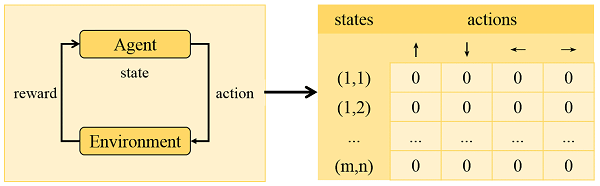
\includegraphics[scale=0.5]{Billeder/tabular-qlearning.png}\\
\caption*{\text{Illustration showing how the tabular q-learning works}}
\end{figure}

Now the challenge is to code this algorithm and define what the states, and the actions for the driving agent should be.

\subsection{Creating the sensors and environment \small\textit{Jacob}} 
We found, that in our game environment the only way to make sensors was in dot form as opposed to rays/vectors, which is the usual way to give the agent an environmental input. The position of our dots is defined by a given angle and length from our car agent, and will return a Boolean value depending on whether it is overlapping with our track border. Checking whether the dots are overlapping is done by seeing if the collision box of the image of the dots are on top of the collision box of the image of the track border. 

The reason dots are used instead of lines / rays is because we cant turn the image collision box only the image itself. Were we to use lines, these would have constant horizontal or vertical hit box regardless of the direction of the agent image and ray image. Thus we chose dots because their image collision box is close to the image itself and the collision box does not need to turn with the agent since its quadratic, as opposed to a rays rectangular hit box.

For any q-learning agent to work, it needs to be given a reward based on its actions, as mentioned earlier a system of sub-goallines were set up on the track to give the agent feedback on its learning process. our reward system was set up as such that for every iteration the standard reward was -1, encouraging the agent to interact with the environment. a negative reward of -100 was given if the agent collided with the wall, and a +100 for crossing these subgoals and the finish line.

\subsection{Creating the agent \small\textit{Jacob}}
With the inputs from the environment in place, the agent then had to be made. Since were using tabular q-learning, the first thing to do was creating a dictionary for all the states our agent could be in. we used the default dictionary from the python module collections. Then the actions of the agent were defined as the following three: turn \textit{left, turn right, forward}. 

The agent is set to always move, with no way to brake or drive backwards. the action forward just means not to turn. The input given to the agent is a tuple of Boolean values describing which dots are colliding with the border. We are using an epsilon-greedy policy with the epsilon being 0.05, meaning that 5 percent of the agents actions is chosen at random, while the rest is chosen with the Quality function. After the action is chosen it is executed and the Q-table is updated. 

Updating the Q-table proved to give a problem since our table is finite and small if the agent is only given a few dots to operate with, it has a limited number of states it can be in. This gives a problem since the agent can be in a given state doing good, and be in that same state while colliding with the border. As a result the Q-table would update with a negative reward to this essentially good state-action. To counter this, we implemented a learning rate of 0.1 for the updating of the Q-table, meaning it would weigh the new value with 10 percent and the existing value in the table with 90 percent, countering these "good state / bad reward"  incidents. Furthermore the quality function had a discount factor of 0.95 to prevent the rewards from escalating towards infinity and to make sure the agent focused a bit more on short-hand rewards.

\subsection{Testing the agent \small\textit{Jacob}}
After creating the agent we wanted to figure out how good / fast it learned to complete the racetrack and how reliable it was based on the configuration of dots. We settled on three models, a two-dot agent, a cone-shaped and a semicircle. Pictures of these are in the appendix. 

In our code, we have the option to switch between testing and training the AI, while the variable Test equals false, the agent trains in the environment as described above, while Test = True however, the agent is tested without the epsilon-greedy policy and without updating its Q-table. it only references to it to decide the appropriate action based on its training. Using this mode enabled us to see whether or not the agent had successfully completed the task finishing the whole track. 
\newpage \section{Results \small\textit{both}} 
The three dot-sensor configurations were tested on the agent and the goal was to complete the whole track a thousand times, a thousand was as a compromise to have enough wins to gather data enough to analyze, while still being small enough for the computation not to take to much time. We graphed the amount of wins over amount of tries:
\begin{figure}[H] \centering
    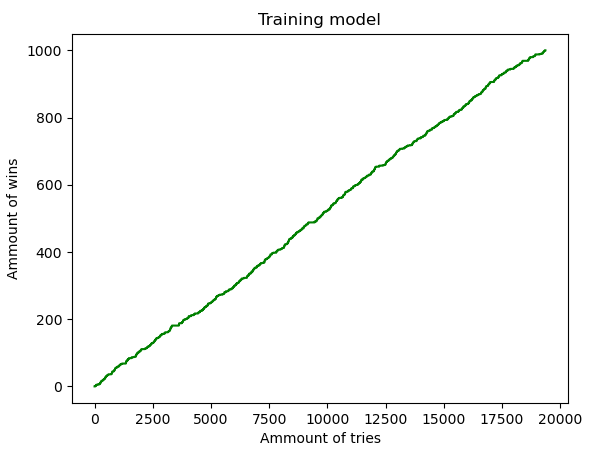
\includegraphics[scale=0.47]{Billeder/2-punkt 19362.PNG}
    \caption{\text{The graph for the two dot configuration. Using 19362 tries to get a thousand wins}}
    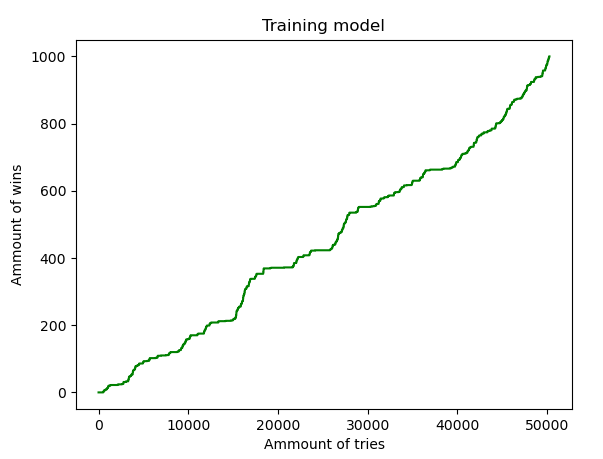
\includegraphics[scale=0.47]{Billeder/Keglesnit 50253.PNG}
    \caption{\textit{The graph for the cone-shaped dot configuration.Using 50253 tries to get a thousand wins}}
    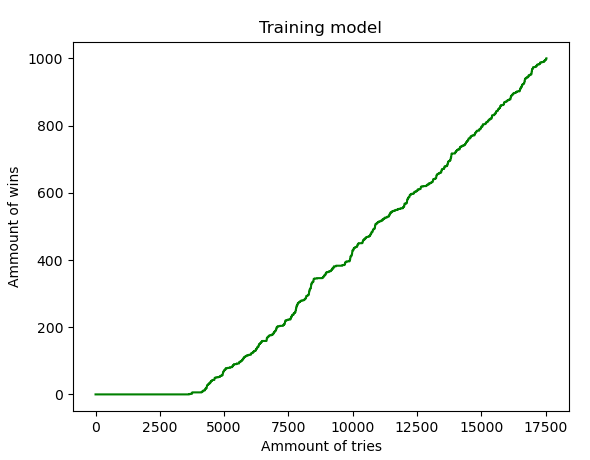
\includegraphics[scale=0.47]{Billeder/Halvcirkel 17538.PNG}
    \caption{\textit{The graph for the semicircle dot configuration. Using 17538 tries to get a thousand wins}}
\end{figure}


\vspace{3mm}
\section{Discussion}
\vspace{3mm}
\subsection{Initial interpretation  \vspace{0.5mm} \small\textit{Jacob}}
What this data show us is actually really interesting as it highlight the pros and cons of each of the three configurations. Looking at the first configuration, it seems to start winning after very few tries, and then it just keeps a steady win-rate the rest of time. For the cone-shaped configuration, the amount of tries before it reaches the thousand wins is substantially larger than the other two configurations. Furthermore it seems to have periods where the win-rate is high and others where it is low. This behavior could be a result of the epsilon exploration / random factor, since the dots in this configuration is so close together, a random move will quickly put the agent in a new state, from which the chosen actions might lead to a border collision. Then the agent would use some tries to 'fix' the Q-table before being able to finish the lap again. Regarding the semicircle, it takes substantially longer before gaining wins, which makes sense, since it has the largest amount of dots, which gives it the by far largest Q-table to fill out. Since the size of the Q-table is determined by the amount of dots: $Qtable_{size}=2^{dots}$ meaning that the three configurations have the following Q-table sizes: $TwoDot = 2^2=4$ and $Cone = 2^7=128$ and $Semicircle = 2^{13}=8192$ This explains why the semicircle is taking a much longer time before it is able to win. 

\subsection{Analysis  \vspace{0.5mm} \small\textit{Jacob}}
Just by looking at the graphs, it is clear that the semicircle is the quickest configuration to reach the desired amount of wins, even though it spends a few thousand tries before getting the first win. This shows that the win-rate of the semicircle is the steepest. To find the win ratio a rough calculation is made, starting from the first win of the three configurations:
\small\[2Dot_{win}=\frac{1000}{19362}=0.05160 \hspace{4.9mm} Cone_{win}=\frac{1000}{50253}=0.020 \hspace{4.9mm} Semicircle_{win} = \frac{1000}{(17538-3000)}=0.06880\]
This rather rough calculation highlight the slope coefficient and thus the difference between the win/lose ratio. The semicircle's high win-rate shows that when its dictionary is adapted, the configuration is more resistant towards the exploration moves.The interesting thing is the cone-shaped configuration, having the most unstable and longest path to the thousand wins. Since the outermost dot to either side is the same as the two dots in the two dot configuration, the remaining dots in the cone shape seems to only cause trouble for the algorithm. The difference between the cone and the semi circle is the dots at an angle of 0 to 45 and 135 to 180, where 90 degrees is straight ahead of the car agent. These dots seems to assist the algorithm a lot better since the semicircle is the fastest configuration of the three.
\subsection{Perspective  \vspace{0.5mm} \small\textit{Kristoffer}}
As in the conclusion in the Analysis, the semicircle was the best form of configuration regarding the agents ability to finish the track. To set this into perspective in the real world of fully self driving cars. The Tesla cars use a similar kind of configuration using cameras with a semicircle that extends a 180 degree peripheral vision. Although at a much more advanced level of algorithms using a deep neural network and visual feedback to analyze the environment, with cameras in the back as well. 

It can be shown in graph 1, 2 and 3 in the results the amount of data needed correlates with the amount of sensors. As the first graph learns pretty fast to get its first win, but is having a hard time finding the optimal way around the track. The 2nd graph takes a bit more time to get its first win, but after the 1000 wins its pretty good at winning fast and efficient. And the 3rd graph with the most amount of sensors, takes a long time for its first win, because of the requisite amount of data is more vast than the others.

Therefore for Tesla and other autonomous car companies pioneers, data is indispensable. This, is also why you might be finding a lot of traffic related captcha's on the internet. Whenever you do a captcha proving you're not a robot to enter a website, you're actually also contributing to gathering the data for a future with fully self driven cars.